\documentclass[11pt]{article}
\usepackage{deauthor,times,graphicx}
\usepackage{amssymb}

\graphicspath{{authorname/}}

%
% Paper size: 6 to 15 pages, single column
% additional info: http://tab.computer.org/tcde/bull_author.html
% deadline: end of January 2016
%

\newcommand{\ex}{$\mathcal{E}$}
\newcommand{\pp}{$\mathcal{P}$}
\newcommand{\ppm}{\mathcal{P}}
\newcommand{\cc}{$\mathcal{C}$}
\newcommand{\ccm}{\mathcal{C}}
\newcommand{\vv}{$\mathcal{V}$}
\newcommand{\vvm}{\mathcal{V}}
\newcommand{\vvt}{$\mathcal{V}$}
\newcommand{\rr}{$\mathcal{R}$}
\newcommand{\rrm}{\mathcal{R}}
\newcommand{\sst}{$\mathcal{S}$}
\newcommand{\ssm}{\mathcal{S}}
%
% S-SMR
\newcommand{\ssmr}{\mbox{S-SMR}}
\newcommand{\ssmrshort}{Scalable SMR}
\newcommand{\ssmrlong}{Scalable State Machine Replication}
%
% DS-SRM
\newcommand{\dssmr}{\mbox{DS-SMR}}
\newcommand{\dssmrshort}{Dynamic S-SMR}
\newcommand{\dssmrlong}{Dynamic Scalable State Machine Replication}
%
% Eyrie and Chirper temporary name (double blind)
\newcommand{\libname}{Nest}    % rename to Eyrie   after paper is accepted
\newcommand{\appname}{Flitter} % rename to Chirper after paper is accepted
%
\newcommand{\rmcast}{reliable-multicast}
\newcommand{\rmdel}{reliable-deliver}
\newcommand{\amcast}{atomic-multicast}
\newcommand{\amdel}{atomic-deliver}

\begin{document}

\title{Strong Consistency at Scale}
 
\author{
  Carlos Eduardo Bezerra\\
  University of Lugano (USI)\\
  Switzerland
  \and
  Le Long Hoang\\
  University of Lugano (USI)\\
  Switzerland
  \and
  Fernando Pedone\\
  University of Lugano (USI)\\
  Switzerland
}

\begin{abstract}
\end{abstract}

\maketitle

\section{Introduction}

\clearpage
\section{System model and definitions}
\label{sec:sysmodel}

\subsection{Processes and communication}

We consider a distributed system consisting of an unbounded set of client processes $\ccm = \{c_1, c_2, ...\}$ and a bounded set of server processes (replicas) $\ssm = \{s_1, ..., s_n\}$. 
Set $\ssm$ is divided into disjoint groups of servers $\ssm_1, ..., \ssm_k$.
Processes are either \emph{correct}, if they never fail, or \emph{faulty}, otherwise. 
In either case, processes do not experience arbitrary behavior (i.e., no Byzantine failures).

Processes communicate by message passing, using either one-to-one or one-to-many communication.
The system is asynchronous: there is no bound on message delay or on relative process speed.
One-to-one communication uses primitives $send(p,m)$ and $receive(m)$, where $m$ is a message and $p$ is the process $m$ is addressed to. 
If sender and receiver are correct, then every message sent is eventually received. 
%
One-to-many communication relies on reliable multicast and atomic multicast,\footnote{Solving atomic multicast requires additional assumptions~\cite{CT96,FLP85}. In the following, we simply assume the existence of an atomic multicast oracle.}
defined in sections~\ref{sec:rmcast} and \ref{sec:amcast}, respectively.
%Atomic broadcast is a special case of atomic multicast in which there is a single group with all servers.


\subsection{Reliable multicast}
\label{sec:rmcast}

To reliably multicast a message $m$ to a set of groups $\gamma$, processes use primitive \rmcast$(\gamma, m)$.
Message $m$ is delivered at the destinations with \rmdel$(m)$.
Reliable multicast has the following properties:

\begin{itemize}

    \item[--] If a correct process \rmcast{}s $m$, then every correct process in $\gamma$ \rmdel{}s $m$ \emph{(validity)}.
    
    \item[--] If a correct process \rmdel{}s $m$, then every correct process in $\gamma$ \rmdel{}s $m$ \emph{(agreement)}.
    
    \item[--] For any message $m$, every process $p$ in $\gamma$ \rmdel{}s $m$ at most once, and only if some process has \rmcast{} $m$  to $\gamma$ previously \emph{(integrity)}.
    
\end{itemize}

\subsection{Atomic multicast}
\label{sec:amcast}

To atomically multicast a message $m$ to a set of groups $\gamma$, processes use primitive \amcast$(\gamma, m)$.
Message $m$ is delivered at the destinations with \amdel$(m)$.
Atomic multicast ensures the following properties:

\begin{itemize}
    
    \item[--] If a correct process \amcast{}s $m$, then every correct process in $\gamma$ \amdel{}s $m$ \emph{(validity)}.
    
    \item[--] If a process \amdel{}s $m$, then every correct process in $\gamma$ \amdel{}s $m$ \emph{(uniform agreement)}.
    
    \item[--] For any message $m$, every process $p$ in $\gamma$ \amdel{}s $m$ at most once, and only if some process has \amcast{} $m$ to $\gamma$ previously \emph{(integrity)}.
    
    \item[--] No two processes $p$ and $q$ in both $\gamma$ and $\gamma'$ \amdel\ $m$ and $m'$ in different orders; also, the delivery order is acyclic \emph{(atomic order)}.
    
\end{itemize}

Atomic broadcast is a special case of atomic multicast in which there is a single group of processes.


%\subsection{Consistency criterion}
%
%Our consistency criterion is linearizability.
%A system is \emph{linearizable} if there is a way to reorder the client commands in a sequence that (i)~respects the semantics of the commands, as defined in their sequential specifications, and (ii)~respects the real-time precedence of commands~\cite{Attiya04}.



\section{State machine replication}
\label{sec:smr}

State machine replication is a fundamental approach to implementing a fault-tolerant service by replicating servers and coordinating the execution of client commands against server replicas~\cite{Lam78, Sch90}. 
The service is defined by a state machine, which consists of a set of \emph{state variables} $\vvm = \{v_1, ..., v_m\}$ 
%that encode the service's state 
and a set of \emph{commands} that may read and modify state variables, and produce a response for the command.
Each command is implemented by a deterministic program.
% whose execution is atomic with respect to other commands.
%The set of variables read by $C$ and the set of variables updated by $C$ are denoted, respectively, by $readset(C)$ and $writeset(C)$.
%The set of all variables read and updated by $C$ is denoted by $var(C)$. 
State machine replication can be implemented with atomic broadcast: commands are atomically broadcast to all servers, and all correct servers deliver and execute the same sequence of commands.

We are interested in implementations of state machine replication that ensure linearizability.
%
Linearizability is defined with respect to a sequential specification.
The \emph{sequential specification} of a service consists of a set of commands and a set of \emph{legal sequences of commands}, which define the behavior of the service when it is accessed sequentially.
In a legal sequence of commands, every response to the invocation of a command immediately follows its invocation, with no other invocation or response in between them.
For example, a sequence of operations for a read-write variable $v$ is legal if every read command returns the value of the most recent write command that precedes the read, if there is one, or the initial value, otherwise.
An execution \ex\ is linearizable if there is some permutation of the commands executed in \ex\ that respects (i)~the service's sequential specification and (ii)~the real-time precedence of commands.
Command $C_1$ precedes command $C_2$ in real-time if the response of $C_1$ occurs before the invocation of $C_2$.

In classical state machine replication, throughput does not scale with the number of replicas: each command must be ordered among replicas and executed and replied by every (non-faulty) replica.
Some simple optimizations to the traditional scheme can provide improved performance but not scalability.
For example, although update commands must be ordered and executed by every replica, only one replica can respond to the client, saving resources at the other replicas.
Commands that only read the state must be ordered with respect to other commands, but can be executed by a single replica, the replica that will respond to the client.

This is a fundamental limitation: while some optimizations may increase throughput by adding servers, the improvements are limited since fundamentally, the technique does not scale.
In the next section, we describe an extension to SMR that under certain workloads allows performance to grow proportionally to the number of replicas.



\section{Scalable State Machine Replication}
\label{sec:scalablesmr}

In this section, we introduce S-SMR, discuss performance optimizations, and argue about S-SMR's correctness.

\subsection{General idea}
\label{sec:generalidea}

S-SMR divides the application state $\vvm$ (i.e., state variables) into $k$ partitions $\ppm_1, ..., \ppm_k$, where for each $\ppm_i$, $\ppm_i \subseteq \vvm$. 
Moreover, we require each variable $v$ in $\vvm$ to be assigned to at least one partition and define $part(v)$ as the partitions that hold $v$. 
Each partition $\ppm_i$ is replicated by servers in group $\ssm_i$.
For brevity, we say that server $s$ belongs to $\ppm_i$ with the meaning that $s \in \ssm_i$, and say that client $c$ multicasts command $C$ to partition $\ppm_i$ meaning that $c$ multicasts $C$ to group $\ssm_i$.
% We also say that $\ppm_i$ does something meaning that servers in $\ssm_i$.
%We also often mention $\ppm_i$ meaning servers in $\ssm_i$.

To execute command $C$, the client multicasts $C$ to all partitions that hold a variable read or updated by $C$.
Consequently, the client must be able to determine the partitions that may be accessed by $C$.
Note that this assumption does not imply that the client must know all variables accessed by $C$, nor even the exact set of partitions.
If the client cannot determine a priori which partitions will be accessed by $C$, it must define a superset of these partitions, in the worst case assuming all partitions.
For performance, however, clients must strive to provide a close approximation to the command's actually accessed partitions.
We assume the existence of an oracle that tells the client which partitions should receive each command.

Upon delivering command $C$, if server $s$ does not contain all variables read by $C$, $s$ must communicate with servers in other partitions to execute $C$. 
Essentially, $s$ must retrieve every variable $v$ read in $C$ from a server that stores $v$ (i.e., a server in a partition in $part(v)$).
Moreover, $s$ must retrieve a value of $v$ that is consistent with the order in which $C$ is executed, as we explain next.
Operations that do not involve reading a variable from a remote partition are executed locally.

In more detail, let $op$ be an operation in the execution of command $C$.
We distinguish between three operation types: $read(v)$, an operation that reads the value of a state variable $v$, $write(v, val)$, an operation that updates $v$ with value $val$,
and an operation that performs a deterministic computation.

Server $s$ in partition $\ppm_i$ executes $op$ as follows.

\begin{itemize}

\item[i)] \underline{$op$ is a $read(v)$ operation.} \\
If $\ppm_i \in part(v)$, then $s$ retrieves the value of $v$ and sends it to every partition $\ppm_j$ that delivers $C$ and does not hold $v$. If $\ppm_i \not\in part(v)$, then $s$ waits for $v$ to be received from a server in a partition in $part(v)$.

\item[ii)] \underline{$op$ is a $write(v,val)$ operation.} \\
If $\ppm_i \in part(v)$, $s$ updates the value of $v$ with $val$; if $\ppm_i \not\in part(v)$, $s$ executes $op$, creating a local copy of $v$, which will be up-to-date at least until the end of $C$'s execution.

\item[iii)] \underline{$op$ is a computation operation.}\\
In this case, $s$ executes $op$.

\end{itemize}


%As we now show, the procedure above does not ensure linearizability.
As we now show, atomically ordering commands and following the procedure above is still not enough to ensure linearizability.
Consider the execution depicted in Figure~\ref{fig:mcastnonlinssmr}~(a), where state variables $x$ and $y$ have initial value of $10$. 
Command $C_x$ reads the value of $x$, $C_y$ reads the value of $y$, and $C_{xy}$ sets $x$ and $y$ to value 20.
Consequently, $C_x$ is multicast to partition $\ppm_x$, $C_y$ is multicast to $\ppm_y$, and $C_{xy}$ is multicast to both $\ppm_x$ and $\ppm_y$. 
Servers in $\ppm_y$ deliver $C_y$ and then $C_{xy}$, while servers in $\ppm_x$ deliver $C_{xy}$ and then $C_x$, which is consistent with atomic order. 
In this execution, the only possible legal permutation for the commands is $C_y$, $C_{xy}$, and $C_x$, which violates the real-time precedence of the commands, since $C_x$ precedes $C_y$ in real-time.

\begin{figure*}
\begin{minipage}[b]{1.0\linewidth} % A minipage that covers the whole width of the page
\centering
      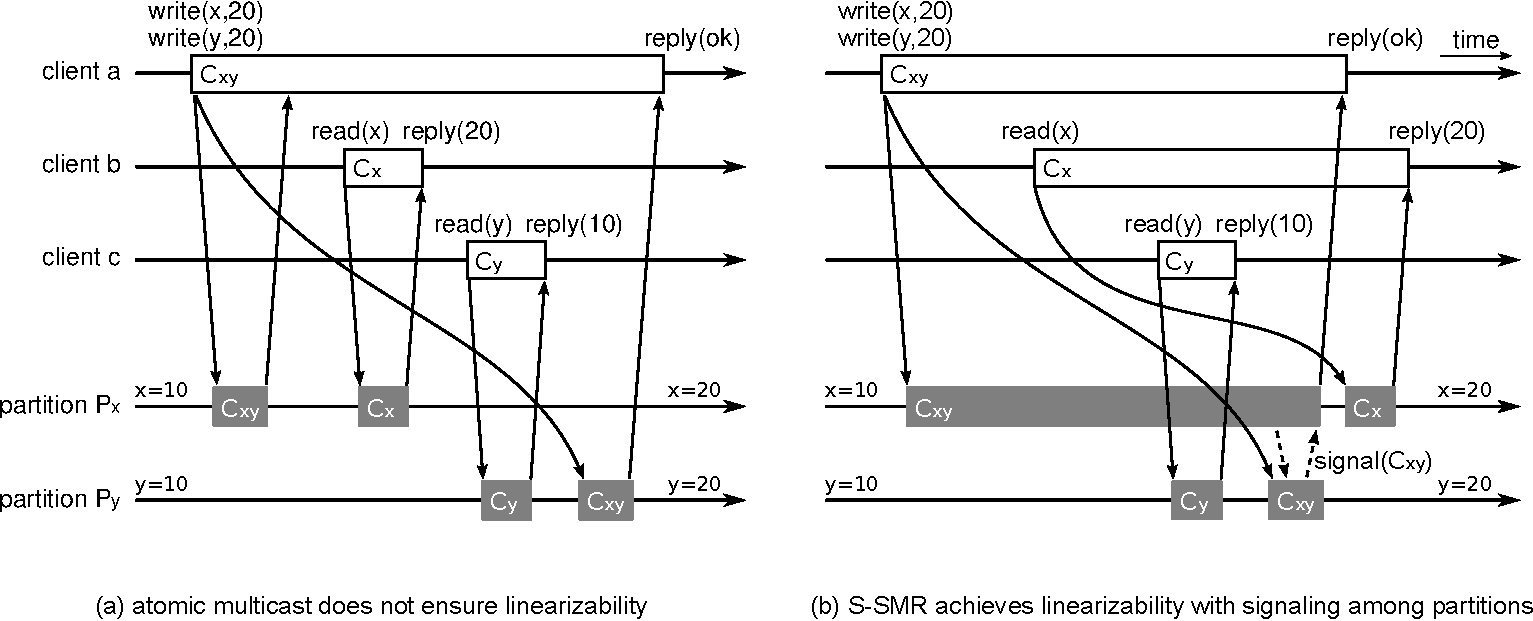
\includegraphics[width=0.85\linewidth]{mcastssmr_nonlin_linsignal_v3}
\end{minipage}
\caption{Atomic multicast and S-SMR. (To simplify the figure, we show a single replica per partition.)}
\label{fig:mcastnonlinssmr}
\end{figure*}

Intuitively, the problem with the execution in Figure~\ref{fig:mcastnonlinssmr}~(a) is that commands $C_x$ and $C_y$ execute ``in between'' the execution of $C_{xy}$ at partitions $\ppm_x$ and $\ppm_y$.
In S-SMR, we avoid such cases by ensuring that the execution of every command is atomic.
%
Command $C$ is \emph{execution atomic} if, for each server $s$ that executes $C$, there exists at least one server $r$ in every other partition in $part(C)$ such that the execution of $C$ at $s$ finishes only after $r$ starts executing $C$.
%
More precisely, let $start(C,p)$ and $end(C,p)$ be, respectively, the time when server $p$ starts executing command $C$ and the time when $p$ finishes $C$'s execution.
Execution atomicity ensures that, for every server $s$ in partition \pp\ that executes $C$, there is a server $r$ in every $\ppm' \in part(C)$ such that \mbox{$start(C,r) < end(C,s)$}.
Intuitively, this condition guarantees that the execution of $C$ at $s$ and $r$ overlap in time.

%Back in Fig.~\ref{fig:mcastnonlinssmr}, each black box represents the execution of a subcommand by servers in the partition: it starts when the first server in the partition begins executing the subcommand and ends when there is no more server executing the subcommand in that partition. We can see that $C_{xy}$ is not execution atomic: there is no time $t$ when some servers $s_x$ in $P_x$ and $s_y$ in $P_y$ are executing it. If it were the case, this example would be impossible to build, since $finish(C_y,s_y) < start(C_{xy}, s_y) < t < finish(C_{xy}, s_x) < start(C_x, s_x)$, which would contradict the fact that $C_x$ precedes $C_y$ in real-time.

Replicas can ensure execution atomicity by coordinating the execution of commands.
After starting the execution of command $C$, servers in each partition send a $signal(C)$ message to servers in the other partitions in $part(C)$.
Before finishing the execution of $C$ and sending a reply to the client that issued $C$, each server must receive a $signal(C)$ message from at least one server in every other partition that executes $C$. 
Because of this scheme, each partition is required to have at least $f+1$ correct servers, where $f$ is the maximum number of tolerated failures per partition; if all servers in a partition fail, service progress is not guaranteed.

Figure \ref{fig:mcastnonlinssmr}~(b) shows an execution of S-SMR. 
In the example, servers in $\ppm_x$ wait for a signal from $\ppm_y$,
therefore ensuring that the servers of both partitions are synchronized during the execution of $C_{xy}$.
Note that the outcome of each command execution is the same as in case (a), but the execution of $C_x$, $C_y$ and $C_{xy}$, as seen by clients, now overlap in time with one another. 
Hence, there is no real-time precedence among them and linearizability is not violated.




\subsection{Performance optimizations}
\label{sec:optm}

Algorithm \ref{alg:ssmr} can be optimized in many ways. 
In this section, we briefly mention some of these optimizations and then detail caching.
\begin{itemize}
\item Server $s$ does not need to wait for the execution of command $C$ to reach a $read(v)$ operation to only then multicast $v$ to the other partitions in $part(C)$. If $s$ knows that $v$ will be read by $C$, $s$ can send $v$'s value to the other partitions as soon as $s$ starts executing $C$.
\item The exchange of objects between partitions serves the purpose of signaling. Therefore, if server $s$ sends variable $v$'s value to server $r$ in another partition, $r$ does not need to receive a signal message from $s$'s partition.
\item It is not necessary to exchange each variable more than once per command since any change during the execution of the command will be deterministic and thus any changes to the variable can be applied to the cached value.
\item Even though all replicas in all partitions in $part(C)$ execute $C$, a reply from a replica in a single partition suffices for the client to finish the command.
\end{itemize}

%Caching is a more elaborate optimization. 
Server $s$ in partition \pp\ can cache variables that belong to other partitions. 
There are different ways for $s$ to maintain cached variables; here we define two techniques: conservative caching and speculative caching. 
In both cases, the basic operation is the following: 
When $s$ executes a command that reads variable $x$ from some other partition $\ppm{}_x$, after retrieving the value of $x$ from a server in $\ppm{}_x$, $s$ stores $x$'s value in its cache and uses the cached value in future read operations.
If a command writes $x$, $s$ updates (or creates) $x$'s local value. 
Server $s$ will have a valid cache of $x$ until (i)~$s$ discards the entry due to memory constraints, or (ii)~some command not multicast to \pp\ changes the value of $x$. 
Since servers in $\ppm_x$ deliver all commands that access $x$, these servers know when any possible cached value of $x$ is stale.
How servers use cached entries distinguishes conservative from speculative caching.
%; what it does not know, however, is whether \pp\ has discarded $x$'s cache. 


Servers in $\ppm_x$ can determine which of its variables have a stale value cached in other partitions. This can be done by checking if there was any command that updated a variable $x$ in $\ppm_x$, where such command was not multicast to some other partition $\ppm$ that had a cache of $x$. Say servers in $\ppm_x$ deliver command $C$, which reads $x$, and say the last command that updated the value of $x$ was $C_w$. Since $x \in \ppm_x$, servers in $\ppm_x$ delivered $C_w$. One way for servers in $\ppm_x$ to determine which partitions need to update their cache of $x$ is by checking which destinations of $C$ did not receive $C_w$. This can be further optimized: even if servers in $\ppm$ did not deliver $C_w$, but delivered some other command $C_r$ that reads $x$ and $C_r$ was ordered by multicast after $C_w$, then $\ppm$ already received an up-to-date value of $x$ (sent by servers in $\ppm_x$ during the execution of $C_r$). If servers in $\ppm$ discarded the cache of $x$ (e.g., due to limited memory), they will have to send a request for its value.


\emph{Conservative caching}: Once $s$ has a cached value of $x$, before it executes a $read(x)$ operation, it waits for a cache-validation message from a server in $\ppm_x$. The cache validation message contains a set of pairs $(var, val)$, where $var$ is a state variable that belongs to $\ppm_x$ and whose cache in $\ppm$ needs to be validated. 
If servers in $\ppm_x$ determined that the cache is stale, $val$ contains the new value of $var$; otherwise, $\perp$, telling $s$ that its cached value is up to date.
If $s$ discarded its cached copy, it sends a request for $x$ to $\ppm_x$.
If it is possible to determine which variables are accessed by $C$ before $C$'s execution, all such messages can be sent upon delivery of the command, reducing waiting time; messages concerning variables that could not be determined a-priori are sent later, during the execution of $C$, as variables are determined.

\emph{Speculative caching}: It is possible to reduce execution time by speculatively assuming that cached values are up-to-date. 
Speculative caching requires servers to be able to rollback the execution of commands, in case the speculative assumption fails to hold. 
Many applications allow rolling back a command, such as databases, as long as no reply has been sent to the client for the command yet. 
The difference between speculative caching and conservative caching is that in the former servers that keep cached values do not wait for a cache-validation message before reading a cached entry; instead, a $read(x)$ operation returns the cached value immediately. 
If after reading some variable $x$ from the cache, during the execution of command $C$, server $s$ receives a message from a server in $\ppm_x$ that invalidates the cached value, $s$ rolls back the execution to some point before the $read(x)$ operation and resumes the command execution, now with the up-to-date value of $x$. 
%This may happen for every variable read by $C$, so $s$ might rollback the execution of $C$ several times until getting it right. 
%To ensure that a correct execution will be done eventually, 
Server $s$ can only reply to the client that issued $C$ after every variable read from the cache has been validated.

%Both caching algorithms depend on the following condition: each partition $\ppm_x$ keeps track of what was the last command $C$ executed by each partition $\ppm$, for each variable $x$ in $\ppm_x$, such that $C$ reads or writes $x$.\fixme{This part is too complicated.}
%Such values are kept by $\ppm_x$ in a table where each entry is $\langle \ppm, x, k \rangle$, where $k$ identifies the last command executed by $\ppm$ that accesses $x$. The initial value of $k$ is $0$ for every partition and every variable. Whenever a command $C$ that accesses $x$ is delivered by $\ppm_x$, it increments the command counter $k$ in $\langle \ppm, x, k \rangle$, for every partition $\ppm$ that delivers $C$. Upon delivery of any command $C'$ that also accesses $x$, $\ppm_x$ checks whether there is any partition $\ppm'$ that $C'$ was multicast to, where the cache of $x$ read by $C'$ will be stale, that is, entries $\langle \ppm_x, x, k \rangle$ and $\langle \ppm', x, k' \rangle$ are such that $k' < k$. Then, $P_x$ sends the cache-validation message(s) to $\ppm'$ accordingly.


\section{Performance evaluation}


\section{Related work}

\section{Final remarks}



\bibliographystyle{ieeetr}
\bibliography{references}

\end{document}
